\chapter{Casos de estudio}\label{cap:casos_estudio}

El capítulo anterior ha descrito el sistema con el que se ejecutan los cinco algoritmos: el simulador de eventos discretos, la función de recompensa y las decisiones de implementación que los materializan. Falta describir \emph{sobre qué} se ejecutan. Este capítulo presenta el catálogo de escenarios empleado en la evaluación y justifica los criterios con los que fue construido.

El conjunto de prueba no se ha diseñado con el único propósito de determinar qué algoritmo obtiene la mayor recompensa media, sino con el de poder atribuir las diferencias observadas a propiedades concretas del problema. Un catálogo de escenarios heterogéneos permitiría constatar que un método rinde más que otro, pero no explicar por qué; y en un problema que combina ventanas de ejecución, coaliciones, restricciones de batería e incertidumbre (Sección~\ref{subsec:mrtau}), esa explicación posee un gran valor. Esta exigencia se traduce en un catálogo de \textbf{360 escenarios repartidos en cinco bloques de 72}, donde cada uno de los bloques varía un único aspecto del problema mientras todo lo demás permanece fijado en una configuración de referencia. Las diferencias observadas dentro de un bloque son atribuibles al factor que ese bloque aísla. La Sección~\ref{sec:casos-comun} describe la configuración común a todos ellos y la Sección~\ref{sec:casos-bloques}, los cinco bloques y el factor que cada uno aísla.

% ===========================================================================
\section{Configuración común de los escenarios} \label{sec:casos-comun}
% ===========================================================================

Todos los escenarios del catálogo comparten una estructura común que se resume en la Tabla~\ref{tab:sustrato} y que se detalla a continuación. Cada uno de ellos constituye una instancia del problema en el sentido de la Definición~\ref{def:instancia}, expresada en el formato YAML que utiliza el simulador (Sección~\ref{sec:mat-arquitectura}).

\begin{table}[t]
\centering
\caption{Configuración común a los 360 escenarios del catálogo.}
\label{tab:sustrato}
\begin{tabular}{ll}
\hline
\textbf{Elemento} & \textbf{Valor} \\
\hline
Grafo                   & Completo, $m+1$ nodos: $m$ nodos de tarea y $1$ nodo de estación \\
Geometría               & Tareas repartidas en $4$ racimos en torno al centro \\
Robots                  & Homogéneos, $\textit{Cap}(i,j)=1$ para todo par, todos parten de la estación \\
Cinemática              & $v_i=1$ (distancia $=$ tiempo) y $\textit{rate-}R_i=1$ \\
Batería                 & $B_i=40$, con nivel inicial completo \\
Estaciones de recarga   & Una sola, situada en el origen \\
Duración de tarea       & $\mathcal{N}(10,\sigma_j^{s})$ en caso de éxito, el fracaso es inmediato \\
Consumo por tarea       & $\textit{rate-}T_j=1$ por unidad de tiempo de ejecución  \\
Reintentos              & Uno: un fracaso es definitivo \\
Horizonte               & $T=40$ \\
Carga por robot         & $L=6$ \\
Ventana de ejecución   & $[t_j^{s},\,t_j^{l}]=[t_0,\;t_0+10+\varepsilon]$ \\
Coalición de referencia & $q_j=1$ \\
\hline
\end{tabular}
\end{table}

\paragraph{Geometría.} El grafo de ubicaciones es completo y las distancias son euclídeas. El nodo $1$, situado en el origen, alberga la única estación de recarga y cada uno de los $m$ nodos restantes alberga una tarea. Las tareas se reparten en \textbf{cuatro racimos} equidistantes del origen, cuyos centros se sitúan en $(0,4)$, $(4,0)$, $(0,-4)$ y $(-4,0)$. Dentro de cada racimo, las tareas se reparten de forma equiespaciada sobre la circunferencia unidad centrada en él. De este modo, la distancia entre la estación y cualquier tarea está comprendida entre $3$ y $5$ unidades, mientras que dos tareas del mismo racimo distan a lo sumo $2$. Esta disposición introduce deliberadamente una tensión entre dos comportamientos razonables: agrupar el trabajo dentro de un racimo, que es barato en desplazamiento, o repartir el equipo entre racimos, que cubre más ventanas simultáneamente. Es una decisión que el algoritmo debe tomar y condicionará su rendimiento.

\begin{figure}[t]
    \centering
    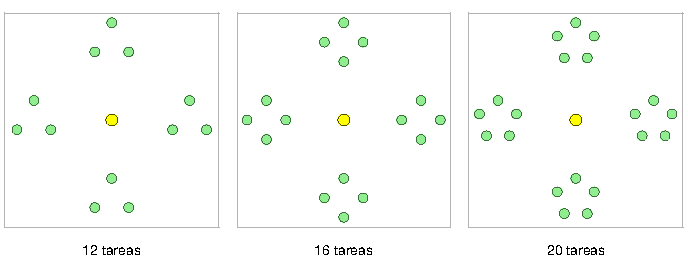
\includegraphics[width=\linewidth]{figures/05_casos_de_estudio/geometria_escenario.pdf}
    \caption{Geometría común a todos los escenarios del catálogo, ilustrada sobre tres instancias en su estado inicial con tres, cuatro y cinco tareas por racimo. Las tareas, en verde, se reparten de forma equiespaciada sobre la circunferencia unidad de cada uno de los cuatro racimos, equidistantes de la estación de recarga, en amarillo, situada en el origen. Como el número de racimos es siempre cuatro, un escenario mayor no añade racimos nuevos, sino que puebla más densamente los ya existentes.}
    \label{fig:geometria}
\end{figure}

\paragraph{Robots y cinemática.} Los robots son idénticos: comparten velocidad, capacidad de batería y tasas de consumo, parten todos de la estación de recarga y son compatibles con todas las tareas, esto es, $\textit{Cap}(i,j)=1$ para todo par $(i,j)$. No se hace uso de la heterogeneidad que admite el modelo formal. Esta es una simplificación deliberada, coherente con el objeto de estudio del trabajo, que es la coordinación entre robots y no la asignación por competencias. La velocidad se fija en $v_i=1$, de manera que las distancias del grafo se leen directamente como tiempos de desplazamiento, y la tasa de consumo al navegar en $\textit{rate-}R_i=1$ unidad de batería por unidad de tiempo. Como la demanda media de una tarea ($10$) coincide con su duración media ($10$), ejecutar y desplazarse cuestan lo mismo por unidad de tiempo: ninguna de las dos actividades resulta más barata que la otra.

\paragraph{Tareas.} Toda tarea tiene una duración media de $10$ unidades de tiempo en caso de éxito, muestreada de $\mathcal{N}(10,\sigma_j^{s})$ y truncada en $0$ (solo se consideran valores positivos). Como la tasa de consumo durante la ejecución es unitaria, una ejecución con éxito gasta tantas unidades de batería como unidades de tiempo ha durado. El fracaso, en cambio, se modela como \textbf{instantáneo}: una ejecución fallida no consume tiempo, pero sí una cantidad fija de $10$ unidades de batería. Es decir, el coste de fallar no es la espera, sino la energía gastada y, sobre todo, la oportunidad perdida, pues no hay reintentos: una tarea que fracasa queda definitivamente sin completar. Esta elección concentra el efecto de la incertidumbre en la calidad de la decisión y evita que el fracaso se convierta simplemente en un retraso. A este fracaso por azar se añade un segundo modo, de naturaleza distinta: si la batería del robot no cubre la duración muestreada, la ejecución se interrumpe en el instante en que se agota. La tarea fracasa igualmente y de forma definitiva, pero el coste ya no es el fijo de $10$ unidades, sino la energía que le restaba al robot.

\paragraph{La definición de dificultad.} La dificultad de un escenario se controla mediante la \textbf{carga por robot}
\begin{equation} \label{eq:carga}
    L \;=\; \frac{1}{n}\sum_{T_j \in \mathcal{T}} q_j,
\end{equation}
esto es, la suma de trabajadores requeridos por tarea entre el número total de robots. Esta cantidad representa el número de tareas que corresponden a cada robot. Todo el catálogo se fija en $L = 6$, fijando además el horizonte en $T = 40$, salvo el bloque que estudia expresamente este factor. El motivo de fijar $L$ y no el número de tareas es que estas dos magnitudes no son intercambiables: si el número de tareas se mantuviera constante al aumentar el equipo, o si el horizonte creciera con él, «más robots» significaría en realidad «menos trabajo por robot» y cualquier tendencia medida frente al tamaño del equipo estaría midiendo holgura en lugar de capacidad de coordinación. Fijando $L$ y $T$, el número de tareas de un escenario queda determinado por el tamaño del equipo y por el tamaño medio de coalición $\bar{q}$ mediante $m = Ln/\bar{q}$, y el tamaño del equipo se convierte en un factor aislable.

\paragraph{La restricción de batería.} La capacidad de batería se fija en $B_i=40$ para todos los robots, que además comienzan el episodio con la batería llena. La cifra no es arbitraria. Un ciclo de trabajo típico consiste en salir de la estación hacia un racimo ($4$ unidades), ejecutar tres tareas ($30$) desplazándose entre ellas ($\approx 2$) y regresar a recargar ($4$), lo que suma unas $40$ unidades. La carga inicial alcanza por tanto para la ejecución de aproximadamente tres tareas. Debido a la carga de trabajo por robot descrita anteriormente, cada robot necesita al menos dos ciclos completos para completar su trabajo, de modo que la recarga pasa a ser una parte obligatoria del problema. Esto responde a una exigencia del propio modelo: la Definición~\ref{def:solucion} incluye la factibilidad energética entre las condiciones que toda solución debe satisfacer, y una capacidad holgada dejaría esa condición sin activarse nunca. La única estación de recarga se sitúa además en el origen, coincidiendo con la posición inicial de los robots.

\paragraph{Ventana y coalición de referencia.} La configuración de referencia emplea la ventana de ejecución más restrictiva de las consideradas, que denominaremos \emph{estrecha}. Para cada tarea se sortean un instante de apertura $t_0 \sim \mathcal{U}\{0,\dots,T\}$ y una perturbación $\varepsilon \sim \mathcal{N}(0,3)$, y la ventana se define como
\begin{equation} \label{eq:ventana-ref}
    [\,t_j^{s},\,t_j^{l}\,] \;=\; [\,t_0,\;\; t_0 + 10 + \varepsilon\,],
\end{equation}
de anchura media $10$, comparable a la duración de la propia tarea. Una ventana así exige que la coalición esté presente en un instante concreto: llegar antes obliga a esperar y llegar tarde inutiliza la tarea. Obsérvese que el horizonte $T$ acota el instante en que las ventanas se \emph{abren}, no la duración del episodio, que termina cuando todos los robots han concluido su misión o agotado su batería. La coalición de referencia es $q_j=1$, es decir, tareas ejecutables por un solo robot; las variantes con coaliciones mayores se estudian en su bloque correspondiente.

\paragraph{Las fuentes de incertidumbre.} Las tres fuentes de incertidumbre introducidas en la Sección~\ref{subsec:mrtau} se controlan de forma conjunta mediante el régimen del escenario, recogido en la Tabla~\ref{tab:regimenes}. El régimen fija la probabilidad de éxito $\rho_j$ y la desviación típica $\sigma_j^{s}$ de la duración en caso de éxito. El resto de parámetros ($\mu_j^s = 10$, $\mu_j^f=0$, $\sigma_j^f=0$) se mantienen siempre fijos. La tercera fuente de incertidumbre, el consumo energético, no se parametriza de forma independiente: como el gasto durante la ejecución es proporcional a su duración, la variabilidad de esta se traslada directamente al consumo. Los dos regímenes de referencia del catálogo son el determinista (\emph{det}) y el estocástico medio (\emph{est}); los dos restantes, incertidumbre leve (\emph{lev}) y fuerte (\emph{fue}), solo aparecen en el bloque que los estudia.

\begin{table}[t]
\centering
\caption{Regímenes de incertidumbre. El régimen determina la probabilidad de éxito y la dispersión de la duración.}
\label{tab:regimenes}
\begin{tabular}{llcc}
\hline
\textbf{Régimen} & & $\rho_j$ & $\sigma_j^{s}$ \\
\hline
\textit{det} & Determinista        & $1{,}00$ & $0$  \\
\textit{lev} & Incertidumbre leve  & $0{,}90$ & $1$  \\
\textit{est} & Incertidumbre media & $0{,}75$ & $3$ \\
\textit{fue} & Incertidumbre fuerte& $0{,}50$ & $5$ \\
\hline
\end{tabular}
\end{table}

% ===========================================================================
\section{Los cinco bloques} \label{sec:casos-bloques}
% ===========================================================================

Sobre la base anterior, el catálogo se organiza en \textbf{cinco bloques de 72 escenarios} cada uno. El bloque~A es el \textbf{control}: lleva íntegra la configuración de referencia y recorre los nueve tamaños de equipo, de $2$ a $10$ robots. Los bloques~B a~E modifican \emph{un único factor} sobre esa referencia y lo hacen para tres tamaños de equipo, $n \in \{2,5,10\}$, de modo que cada uno de ellos se compara contra las celdas correspondientes del bloque de control. La Tabla~\ref{tab:bloques} resume la estructura resultante.

\begin{table}[t]
\centering
\caption{Estructura del catálogo. Cada bloque aísla un único factor y aporta 72 escenarios. La columna de estructura indica el diseño factorial que los genera: niveles del factor $\times$ tamaños de equipo $\times$ regímenes $\times$ instancias; en el bloque~E el factor es el propio régimen, de ahí que no aparezca como un término independiente.}
\label{tab:bloques}
\begin{tabular}{llll ccc}
\hline
\textbf{Bloque} & \textbf{Factor aislado} & \textbf{Niveles} & \textbf{Estructura} & \textbf{det} & \textbf{est} & \textbf{Total} \\
\hline
A (control) & Tamaño del equipo $n$ & $2,\dots,10$          & $9\times 2\times 4$          & 36 & 36 & 72 \\
B & Forma de $[t_j^{s},t_j^{l}]$   & 3 ventanas            & $3\times 3\times 2\times 4$  & 36 & 36 & 72 \\
C & Carga por robot $L$            & $3$, $4$, $8$         & $3\times 3\times 2\times 4$  & 36 & 36 & 72 \\
D & Coalición $q_j$                & $q2$, $qm$            & $2\times 3\times 2\times 6$  & 36 & 36 & 72 \\
E & Régimen $\rho_j$               & $1$, $0{,}9$, $0{,}75$, $0{,}5$ & $4\times 3\times 6$ & 18 & 54 & 72 \\
\hline
\multicolumn{4}{l}{\textbf{Total}} & \textbf{162} & \textbf{198} & \textbf{360} \\
\hline
\end{tabular}
\end{table}

Los bloques~A, B, C y D se reparten \textbf{a partes iguales entre el régimen determinista y el estocástico}: cada escenario descrito se instancia en ambos regímenes, lo que permite leer cualquier comparación por separado en uno y otro. Esta simetría es deliberada, pues el efecto de la incertidumbre sobre los distintos algoritmos es uno de los objetos centrales del estudio y agregar ambos regímenes en una sola cifra podría ocultarlo. El bloque~E constituye la \textbf{única excepción}: el bloque se centra en el estudio de la incertidumbre y el régimen determinista es uno de sus cuatro niveles, el correspondiente a $\rho_j=1$. En este bloque, los escenarios se dividen a partes iguales entre los 4 niveles de incertidumbre. La regla se cumple, por tanto, en $288$ de los $360$ escenarios, y el catálogo completo queda repartido en $162$ escenarios deterministas y $198$ estocásticos.

Cada combinación de parámetros específica del escenario aparece presente además en varias \textbf{instancias} independientes; cuatro en los bloques A, B y C, seis en los bloques D y E. La diferencia existente entre las instancias de una misma combinación de parámetros aparece en los sorteos de las ventanas de ejecución descritos en la Ecuación~\eqref{eq:ventana-ref}. Estas instancias no son repeticiones de la misma ejecución, sino problemas distintos con una misma configuración y permitirá distinguir un comportamiento sistemático de uno particular a una instancia concreta.

La semilla con la que se generan los sorteos de un escenario se deriva exclusivamente del \textbf{tamaño del problema y del número de instancia}, y no del régimen, la forma de la ventana ni la coalición. Dos escenarios con el mismo número de robots, el mismo número de tareas y el mismo índice de instancia comparten, en consecuencia, la geometría y los mismos valores sorteados de $t_0$ y $\varepsilon$, que se extraen siempre en idéntico orden. La comparación entre dos niveles de una característica es así \textbf{pareada tarea a tarea} y no solo escenario a escenario: cuando se contrastan dos formas de ventana, por ejemplo, los plazos de cada tarea son literalmente los mismos números en ambos ficheros, de modo que la diferencia observada solo puede atribuirse al factor variado.

Cada escenario se identifica mediante un nombre de fichero que codifica su posición en el catálogo, con la forma
\begin{center}
\texttt{esc\_\{bloque\}\_r\{robots\}\_n\{tareas\}\_}\texttt{\{ventana\}\_ \\
\{régimen\}\_\{coalición\}\_i\{instancia\}}
\end{center}
donde \texttt{esc\_A\_r05\_n030\_E\_est\_q1\_i3} representa la tercera instancia del bloque A con cinco robots y treinta tareas, ventana estrecha, régimen estocástico medio y tareas de un solo trabajador. El catálogo completo se genera de forma determinista a partir de la especificación anterior, de modo que los $360$ ficheros pueden reconstruirse íntegramente sin ambigüedad.

Los apartados que siguen describen cada bloque y el factor que aísla.

% ---------------------------------------------------------------------------
\subsection{Bloque A: El tamaño del equipo} \label{subsec:casos-bloqueA}
% ---------------------------------------------------------------------------
El bloque de control recorre los nueve tamaños de equipo, de $2$ a $10$ robots, con la configuración de referencia completa. Al mantenerse la carga en $L=6$, el número de tareas acompaña al del equipo ($m=6n$, entre $12$ y $60$ tareas), de modo que todos sus escenarios plantean la misma dificultad nominal y las diferencias entre tamaños son atribuibles a la coordinación y no a la holgura. Es el bloque que evalúa cómo responde el rendimiento de los algoritmos al tener que soportar una mayor coordinación, es decir, más robots.

% ---------------------------------------------------------------------------
\subsection{Bloque B: La ventana de ejecución} \label{subsec:casos-bloqueB}
% ---------------------------------------------------------------------------
Este bloque sustituye la ventana estrecha de referencia por otros tres tipos de ventana, construidos a partir de los mismos sorteos $(t_0,\varepsilon)$ y representados en la Figura~\ref{fig:ventanas}:
\begin{itemize}
    \item \textbf{Solo plazo}, $[\,0,\;t_0+10+\varepsilon\,]$: conserva \emph{exactamente} los mismos instantes de cierre que la ventana de referencia, pero abre todas las tareas desde el comienzo del episodio.
    \item \textbf{Escalonada}, $[\,0,\;\tfrac{g}{4}T+\varepsilon\,]$, donde $g \in \{ 1, 2, 3, 4\}$ identifica el racimo al que pertenece la tarea: los cuatro racimos vencen sucesivamente a un cuarto, la mitad, tres cuartos y la totalidad del horizonte.
    \item \textbf{Ancha}, $[\,0,\;T+10+\varepsilon\,]$: el plazo deja de ser una restricción efectiva y el problema se reduce a un problema de recorrido.
\end{itemize}
El contraste entre la ventana estrecha de referencia y la de solo plazo merece atención particular, porque es el que aísla un factor que la literatura de asignación con ventanas rara vez separa: ambas comparten los mismos plazos y difieren únicamente en si la tarea está disponible desde el instante inicial o hay que esperar a que se abra. Lo que las distingue es, por tanto, la \textbf{espera obligatoria}, que introduce un recurso adicional, el tiempo muerto de un robot comprometido con una tarea que aún no puede comenzar, inexistente cuando la ventana solo impone una fecha límite. La ventana escalonada, por su parte, no exige esperar pero sí ordenar el trabajo por urgencia de racimo, y la ancha elimina toda limitación temporal.

\begin{figure}[t]
    \centering
    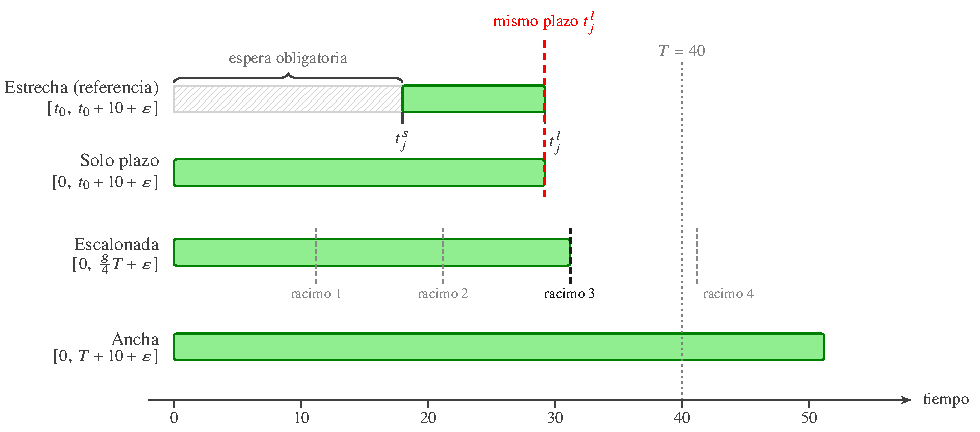
\includegraphics[width=\linewidth]{figures/05_casos_de_estudio/ventanas.pdf}
    \caption{Las cuatro tipologías de ventana de ejecución, derivadas de los mismos sorteos $t_0$ y $\varepsilon$ para una misma tarea, perteneciente en el ejemplo al tercer racimo. La ventana estrecha y la de solo plazo cierran \emph{exactamente} en el mismo instante y difieren únicamente en la espera obligatoria que impone la primera, lo que aísla la espera como factor. En la escalonada el plazo depende del racimo: las marcas discontinuas señalan los cuatro cierres posibles y la destacada es la que corresponde a la tarea representada. La ventana ancha no impone acoplamiento temporal alguno.}
    \label{fig:ventanas}
\end{figure}


% ---------------------------------------------------------------------------
\subsection{Bloque C: La carga por robot} \label{subsec:casos-bloqueC}
% ---------------------------------------------------------------------------
Este bloque evalúa la flexibilidad de los algoritmos en función de la dificultad, medida como la carga por robot. Los niveles $L \in \{3,4,8\}$ se recorren manteniendo el horizonte fijo ($T=40$), lo que sitúa a los escenarios por debajo ($L=3$, $L=4$) y por encima ($L=8$) del punto de operación de referencia. Es el bloque de escenarios más dispares en tamaño, desde $6$ hasta $80$ tareas, y el que permite comprobar si el orden entre algoritmos se mantiene cuando el problema pasa de holgado a saturado.

% ---------------------------------------------------------------------------
\subsection{Bloque D: Las coaliciones} \label{subsec:casos-bloqueD}
% ---------------------------------------------------------------------------
Las tareas de un solo trabajador se sustituyen aquí por tareas \emph{multi-robot}, en dos variantes: $q2$, en la que todas las tareas requieren exactamente dos robots, y $qm$, en la que el número de trabajadores sigue un patrón cíclico $1$-$2$-$3$ con el mismo tamaño medio de coalición, $\bar q = 2$. La pareja está construida así a propósito: ambas variantes imponen idéntica carga agregada y difieren solo en su homogeneidad, lo que separa el efecto de \emph{cooperar} del de cooperar en grupos \emph{de tamaño variable}. Para conservar la carga por robot, el número de tareas se reajusta según $m=Ln/\bar q$, de modo que estos escenarios tienen la mitad de tareas que los de referencia y cada una de ellas es el doble de pesada; conviene tenerlo presente al interpretar la métrica, pues cada tarea completada vale aquí el doble en la fracción final. Los tamaños de equipo empleados son $n \in \{3,6,10\}$, elegidos para que el número de tareas resultante se reparta de forma equilibrada entre los cuatro racimos.

% ---------------------------------------------------------------------------
\subsection{Bloque E: El nivel de incertidumbre} \label{subsec:casos-bloqueE}
% ---------------------------------------------------------------------------
El nivel completo de incertidumbre se recorre sobre los cuatro regímenes descritos en la Tabla~\ref{tab:regimenes}, desde el determinista hasta la incertidumbre fuerte con $\rho_j=0{,}5$, para tres tamaños de equipo. Mientras que el resto de bloques contrasta dos regímenes extremos, este permite observar la \emph{transición}: cómo se degrada el rendimiento de cada algoritmo conforme la incertidumbre crece de forma gradual y si esa degradación depende del tamaño del equipo.

